\chapter{Introducción}

\bigskip
Toda observación de cualquier fenómeno astronómico con cierto interés, requiere de múltiples trabajos laboriosos, tareas  como  la orientación, monitorizar la  meteorología, así como operaciones de control para cada componente del observatorio, ya sea la montura del telescopio, la cámara CCD, el enfocador, la rueda de filtros etc., todo ello requiere gran cantidad de trabajo por parte del operador, asumiendo también una perdida de tiempo útil y un riesgo que se puedan producir errores humanos o accidentes, que pongan en peligro la noche de observación.

\bigskip
Muchas de las operaciones siguen patrones claros, y tienen relación con el estado sensor o periférico, podemos definir rutinas automáticas,
que agilicen los trabajos inherentes a la observación. 

\bigskip
Un ejemplo claro puede ser la decisión de abrir o cerrar la cúpula en un momento dado en función de los datos arrojados por la estación meteorológica, o la decisión de corregir el foco según el perfil de brillo obtenido para las estrellas presentes en las imagenes tomadas por la cámara CCD.

\bigskip
En el mercado existen ya gran cantidad de recursos que se encargan de automatizar las tareas antes citadas, sin embargo, el acceso a estos recursos es caro y no todo aficionado a la astronomía puede permitírselo. Incluso pudiendo el nivel de sofisticación y complejidad
de algunos modelos complican su manejo y por tanto el disfrute en la observación.


\newpage
\bigskip
Para poner en contexto el proyecto, se  propone un recorrido por algunos de las ciencias, tecnologías y disciplinas que toman especial  protagonismo a lo largo de las siguientes páginas.


\begin{itemize}
  \item {Astronomía}
  \item {Instrumental astronómico}
  \begin{itemize}
    \item{Telescopios}
    \item{Enfocadores}
    \item{Cámara y CCD}
    \item{Imagenes FITS}
  \end{itemize}
  \item {Hardware libre}
   \begin{itemize}
     \item{Arduino}
     \item{Raspberry Pi}
   \end{itemize}
  \item {Observatorios remotos}
   \begin{itemize}
     \item{ASCOM}
     \item{INDI}
     \item{Clientes remotos}
  \end{itemize}
  \item {Software procesamiento imagenes astronómicas}

\end{itemize}



\begin{figure}[b]
\centering
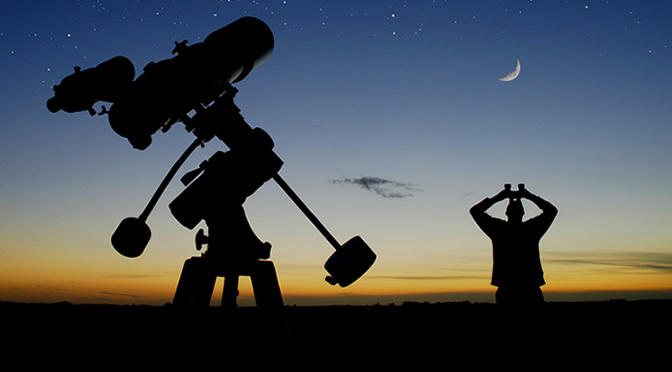
\includegraphics[width=0.7\linewidth]{../images/observatorio_amateur}
\caption[Observatorio Amateur]{http://astrocienciasecu.blogspot.com.es/}
\label{fig:observatorio_amateur}
\end{figure}


\newpage
\section{La Astronomía}

\bigskip
Significa literalmente el estudio de las \textbf{leyes} que rigen los \textbf{astros} o cuerpos celestes, según su etimología griega y latina.

\bigskip
Definiéndola formalmente como:

\begin{quote}``\textit{Ciencia que se ocupa del estudio de los cuerpos celestes del universo, incluidos los planetas y sus satélites, los cometas y meteoritos, las estrellas y la materia interestelar,
  los sistemas de materia oscura, estrellas, gas y polvo llamados galaxias y los cúmulos de galaxias; por lo que estudia sus movimientos y fenómenos ligados a ellos.}''
\newline(\href{https://es.wikipedia.org/wiki/Astronom%C3%ADa}{https://es.wikipedia.org/wiki/Astronomia})
\end{quote}

\bigskip
Pudiendo afirmar que fue la ciencia más remota por el impacto visual y emocional que causó en nuestros antepasado, llegando a captar la atención de tal forma como para pararse a estudiar y analizar el funcionamiento de los objetos suspendidos en el firmamento,fenómenos que no conseguían explicar por completo, y por eso los llegaban a divinizar en múltiples culturas.

\bigskip
Así, Rah, fue el Dios Sol para los egipcios e Isis, la diosa Luna;
y la posición de planetas y estrellas los llevaron a predecir el futuro en base a su ubicación espacial, lo que originó la astrología.

\bigskip
Por tanto la  astronomía es una ciencia antigua y moderna a la vez. \newline
Antigua porque se remonta prácticamente al origen de la humanidad.\newline
Moderna porque nos proporciona uno de los campos de estudio e investigación más avanzados.

\bigskip
Ciencia cargada de múltiples misterios que a día de hoy se siguen manteniéndose, con múltiples  interrogante, como por ejemplo,  si existe vida fuera de la Tierra, o si somos la única civilización
inteligente.


\begin{figure}[b]
\centering
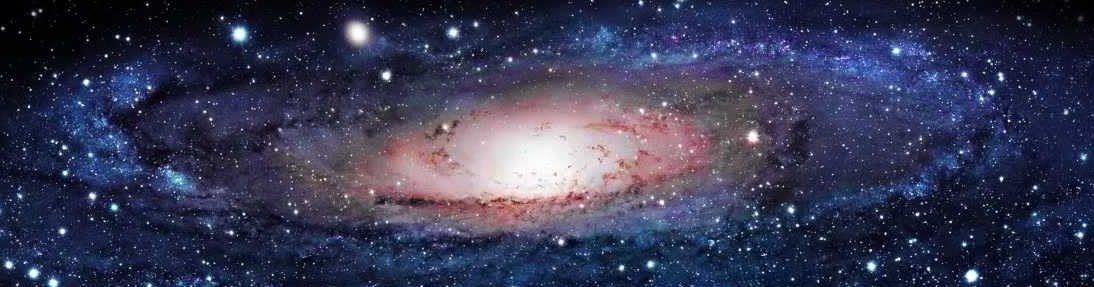
\includegraphics[width=0.9\linewidth]{../images/astrofooter}
\caption[Galaxia]{http://androidayuda.com/app/uploads/2016/03/Astrologia.jpg}
\label{fig:astrofooter}
\end{figure}


\subsection{Astronomía Antiguas}

\bigskip
Civilizaciones tan antiguas como la asiria, babilónica o  sumeria, ya comenzó a transmitirnos los primeros conocimientos sobre el universo que conocemos gracias a la difusión realizada por la cultura griega.

\bigskip
Otros pueblos poderosos también le dieron especial interés a la astronomía y cosmología, pudiendo señalar a los egipcios, sin olvidar a  los pueblos del lejano oriente, los chinos, japoneses y los hindúes.

\bigskip
Teniendo especial importancia los conocimientos astronómicos de los egipcios, dado para ellos el estudio del cielo y elaborar su 
(\href{https://es.wikipedia.org/wiki/Calendario_egipcio}{\textbf{calendario egipcio}} les era de vital importancia dado que les permitía controlar los ciclos de la agricultura y prever la gran inundación del río Nilo, que daba comienzo al año.

\bigskip
En el nuevo Mundo, los mayas llegaron a alcanzar importantes conocimientos de los cuerpos celestes elaborando un calendario donde
el año \textbf{maya} difiere del actual en menos de cinco minutos.
\newline

\bigskip
Los incas se consideraban a sí mismos descendientes del Sol y los aztecas adoraban al dios \textbf{Huitzilopochtli}, símbolo del Sol
que amanecía cada mañana para hacer la lucha con sus hermanas, las estrellas
y así imponer su reinado diurno.
\newline

\bigskip
Moría cada atardecer y tras recuperar las fuerzas, volvía a la madre Tierra, para repetir el ciclo del día.

\bigskip
Se presume que ya en el  siglo III a,C, el astrónomo griego \textbf{Aristarco de Samos} ~\cite{Arist} ya puso en duda todo el modelo geocéntrico griego y postuló que la Tierra gira en 24 horas y se traslada en torno al Sol en un año. Realizando también dibujos de las órbitas planetarias en el orden que ahora las conocemos.

\bigskip
\textbf{Pitágoras} ~\cite{Pitagoras} en el siglo VI  a.C. ya tenia ideas sobre los movimientos, de rotación  de la Tierra en torno a su eje, de traslación en torno al Sol y conocimiento de la esfericidad de la Tierra, Luna y Sol.  ~\cite{AstroAnti}

\newpage

\subsection{Astronomía Moderna}

\bigskip
Se dice que la Astronomía moderna ~\cite{AstMod} inicia su desarrollo con Nicolás  (1473-1543)  quien el año de su muerte publica un trabajo de importancia capital, \textbf{De revolutionibus orbium caelestium} ~\cite{Copernico}.

\bigskip
 La Tierra ya no permanece inmóvil en el centro del universo, sino que está animada de un doble movimiento: de rotación sobre ella misma, en 24 horas, y de revolución alrededor del Sol, en un año. También establece movimientos similares para los planetas y satélites, configurando un sistema más simple que el de Ptolomeo, aunque mantiene como él los movimientos circulares.

\bigskip
Una aportación fundamental en el desarrollo de la nueva es debida a Tycho Brahe (1546-1601) ~\cite{Tycho} teniendo gran importancia sus observaciones, y  sentando las bases que facilitarían a su discípulo Johannes Kepler (1571-1630) ~\cite{Kepler}, el descubrimiento de las famosas leyes que rigen el movimiento, el abandono de las órbitas circulares y la ruptura definitiva con unos conceptos tradicionales que estaban profundamente arraigados. 

\bigskip
La publicación de los Principia en 1685 por Isaac Newton (1643-1727) ~\cite{Newton} marca uno de los puntos culminantes de la ciencia moderna, las leyes de Kepler quedan incluidas en un sistema físico que explica una serie de fenómenos naturales como las estaciones del año, las mareas, los movimientos de los astros, mediante un conjunto consistente de leyes de carácter general que podían ser probadas en un laboratorio.

\bigskip
En este punto la Astronomía y la Astrología inician caminos diferentes y desde entonces no tienen ningún punto común.

\bigskip
Mientras que la primera busca una explicación mecanicista de los fenómenos naturales aplicando leyes formuladas consistentemente y controladas en laboratorio, la Astrología tiene como objetivos la realización de predicciones sobre la personalidad de los individuos y de los sucesos, basándose en las posiciones relativas de los astros.  ~\cite{astrologia}

\bigskip
Durante el siglo XVIII tienen lugar aportaciones importantes en el campo de la astronomía observacional que constituyeron la base observacional para el estudio del Universo a gran escala. Ch. Messier, presentó en la Academia de Ciencias de Francia en 1771, el primer catálogo de y asociaciones de cúmulos estelares, descubiertas u observadas por él. ~\cite{messier}

\bigskip
El descubrimiento de la fotografía y el progreso en la elaboración de emulsiones fotográficas, produjo un rápido avance en la aplicación de la astronomía. En 1863 Huggins obtiene los primeros espectros estelares ~\cite{analisispectal} abriendo una nueva era en la Astronomía. ~\cite{huggins}


\bigskip
Desde finales del siglo XIX y principios del XX la Física pasa a desempeñar un papel decisivo en la interpretación de los fenómenos astronómicos. La Astrofísica ~\cite{astrofisica} adquiere una progresiva importancia sobre la astronomía clásica, utilizando en la actualidad ambos términos de forma sinónima.


\subsection{Astronomía en la actualidad}

Viendo el recorrido de esta ciencia en el pasado nos preguntamos por su repercusión en en la sociedad presente. Poniendo en valor los beneficios que tiene su estudio y los interrogantes que a día de hoy científicos de todo el mundo trabajan por por dar respuesta.  \cite{beneficiosastro}

\bigskip
Los beneficios que obtiene nuestra sociedad los podemos catalogar según su alcance en:


\bigskip
Beneficio puramente científico, el impulso por el conocimiento que ha caracterizado desde siempre al ser humano.Responder interrogantes existenciales como “¿De dónde venimos?, ¿a dónde vamos?”.

\bigskip
Buscar la expansión del Universo, el Big Bang, Agujeros Negros.. son conceptos cosmológicos complejos, que poco a poco  llegan a la sociedad.
 Para ello ha sido necesario  muchos esfuerzos por parte de muchos investigadores, a lo largo de décadas, junto con el desarrollo de instrumentos cada vez más sofisticados, para llegar a estas conclusiones. 

\bigskip
Siendo importante el beneficio puramente científico, no debemos olvidar otros beneficios más próximos a la sociedad. Por una parte, los descubrimientos astronómicos han sido elementos clave para el avance de la Física. 

\bigskip
Como ejemplos tangibles, los astrónomos hemos impulsado el desarrollo de numerosas tecnologías que posteriormente han tenido aplicaciones en la sociedad, tenemos varios ejemplos:   \cite{beneficiosastro2}

\bigskip
Los detectores CCD que usan nuestras cámaras de fotos fueron inventados en 1969, pero lograron desarrollarse rápidamente gracias a sus aplicaciones en instrumentos astronómicos. \newline
 
Los detectores de  rayos X que existen en los aeropuertos fueron desarrollados  para aplicar los  conocimientos  adquiridos en los detectores de rayos X para instrumentos astronómicos. 
Sin olvidad la televisión satélite, con la que estamos familiarizados y usamos a diario en nuestra vida cotidiana.  


\newpage

\subsection{Astronomía amateur}

La astronomía amateur es la realizada por astrónomos no profesionales, normalmente sin realizar formación reglada, y que su interés primordial esta en
está en aprender y conocer esta ciencia, asistir a charlas, ir a quedadas astronómicas y compartir esta afición con otras personas.

\bigskip
La labor de este conjunto es muy valorada, dado que se suelen compartir sus trabajos, colaborando con asociaciones de astronomía y nutriendo de numeroso material muy variopinto, (observaciones desde múltiples ubicaciones, momentos en el tiempo o equipo de observación diferente), ampliando así la cantidad de muestras. No pudiendo llevar más razón el refranero español, \textit"Más ven cuatro ojos que dos"

\bigskip
Todo este trabajo posteriormente puede ser organizado por profesionales y pueden sacar conclusiones así como también se encargan de verificar los descubrimientos científicos presentados por los profesionales. 

\bigskip
Sin olvidar la labor divulgativa. Muchos astrónomos aficionados dedican tiempo y energías impartiendo conferencias no sólo en sus agrupaciones, sino también en actos culturales promovidos por municipios o en escuelas básicas, medias o universitarias. 

\bigskip
Uno de los perfiles más visuales, es el de la astro-fotografía ~\cite{AstroFoto}, que consiste  en la captación fotográfica de las imágenes de los cuerpos celestes. Teniendo gran valor artístico en muchos casos.

\bigskip
En muchas ocasiones, la frontera entre astrónomos profesionales y amateur es muy tenue porque algunos de ellos han contribuido de manera destacada al  conocimiento del cielo nocturno.


\begin{figure}
\centering
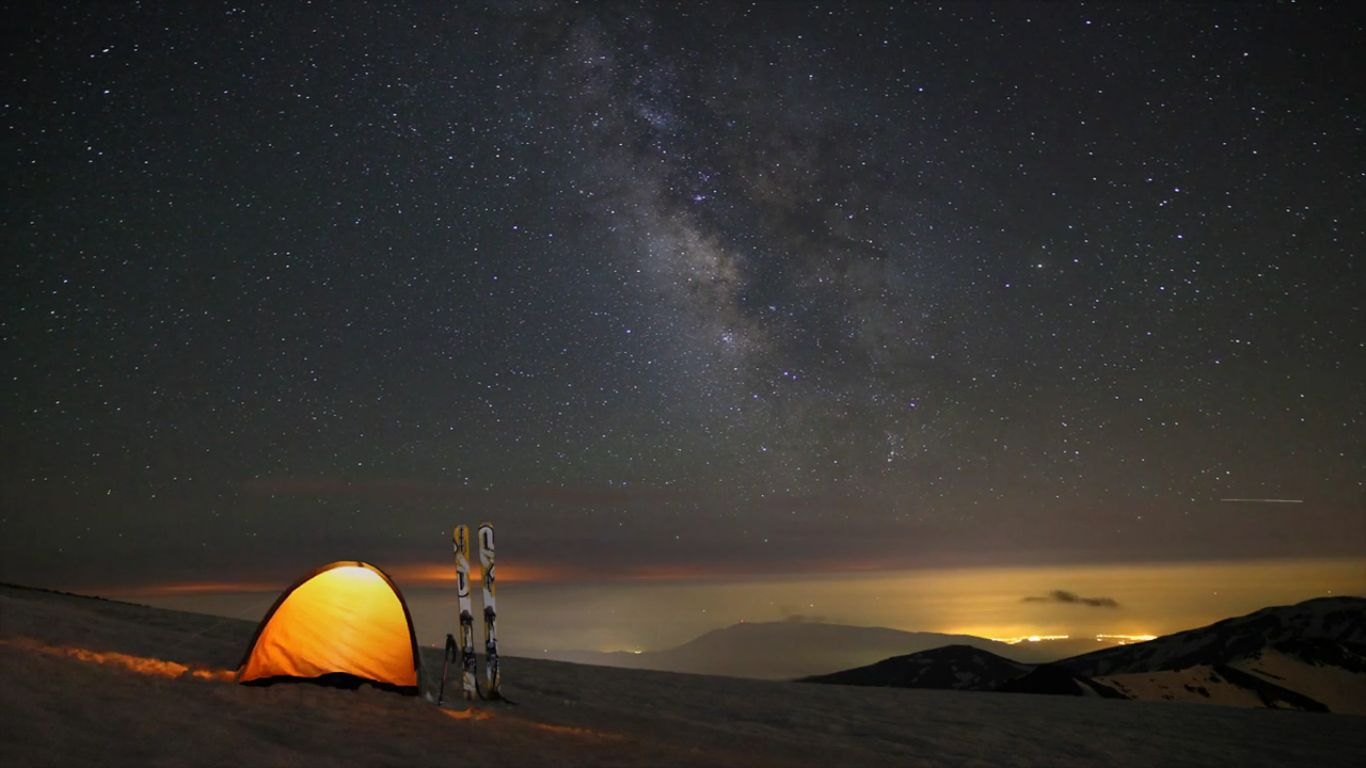
\includegraphics[width=0.7\linewidth]{../images/nightsky}
\caption{Isidro Villo isidro.villo@upct.es}
\label{fig:nightsky}
\end{figure}


\newpage

\newpage
\section{Instrumental Astronómico}

Como ya he enunciado anteriormente la astronomía también está relacionada  con una serie de herramientas e instrumentos básico, que permiten expandir los sentidos del observador,
permitiéndole llegar a ver objetos más lejanos y detectar más características de ellos.  

\subsection{Telescopios}

Un telescopio es un instrumento que, básicamente, pretenden recoger la mayor cantidad posible de energía en forma de luz emitida por un objeto situado más allá de la atmósfera y concentrarla, para así permitir la detección de imágenes que a simple vista son inapreciables. \cite{Telescopio}

\bigskip
Para ello se vale de un sistema óptico principal, que puede ser de lentes o de espejos.


\begin{figure}[!ht]
	\begin{center}
		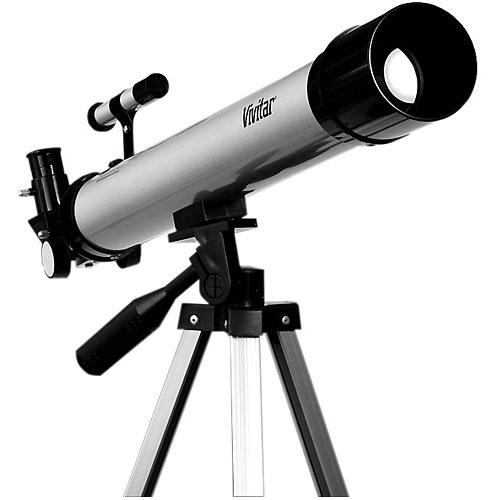
\includegraphics[width=0.6\textwidth]{../images/telescopio2.jpg}
			\caption[Telescopio]{Telescopio (\href{http://cienciaaaoa.blogspot.com.es/2014/11/instrumentos-cientificos_20.html}{Instrumentos-cientificos}).}
		\label{fig:telescop}
	\end{center}
\end{figure}

\bigskip
 Es una herramienta fundamental en astronomía, y cada desarrollo o perfeccionamiento de este instrumento ha permitido avances en nuestra comprensión del Universo.



\bigskip
Debemos agradecer este instrumento en gran parte a \textit{Galileo}, cuyos avances permitieron usar el aparato como instrumento astronómico. 

\bigskip
Existen dos grandes divisiones entre los telescopios, según el tipo de objetivo que utilizan: los \textbf{reflectores} y los \textbf{refractores}. 

\bigskip
Los reflectores se constituyen de un espejo principal (espejo primario u objetivo), el cual no es plano como los espejos convencionales, sino que fue provisto de cierta curvatura (idealmente parabólica) que le permite concentrar la luz en un punto.

\begin{figure}[h]
	\centering
	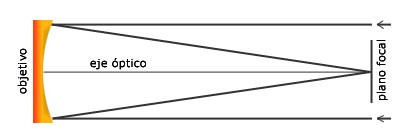
\includegraphics[width=0.7\linewidth]{../images/refrector}
	\caption[Telescopio]{Reflector - www.astrored.net/astronomiasur}
	\label{fig:refrector}
\end{figure}

Existen varios diseños de este tipo de telescopios. Los mas conocidos entre los aficionados son el \textbf{reflector Newtoniano} y el \textbf{reflector Schmidt-Cassegrain}. 




\bigskip
Los refractores poseen como objetivo una lente (o serie de lentes, la cantidad varía según el diseño y calidad) que de forma análoga al funcionamiento de una lupa, concentran la luz en el plano focal. 


\begin{figure}[h]
	\centering
	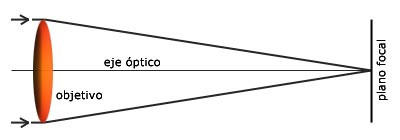
\includegraphics[width=0.7\linewidth]{../images/refractor}
		\caption[Telescopio]{Refractor -  www.astrored.net/astronomiasur }
	\label{fig:refrector}
\end{figure}



\subsection{Cámaras CCD}

Un dispositivo de carga acoplada (en inglés \textbf{Charge-Coupled Device}, conocido también como \textbf{CCD}), es un circuito integrado que contiene un número determinado de condensadores enlazados o acoplados. Bajo el control de un circuito interno, cada condensador puede transferir su carga eléctrica a uno o a varios de los condensadores que estén a su lado en el circuito impreso.

\bigskip
\begin{figure}[!ht]
	\begin{center}
		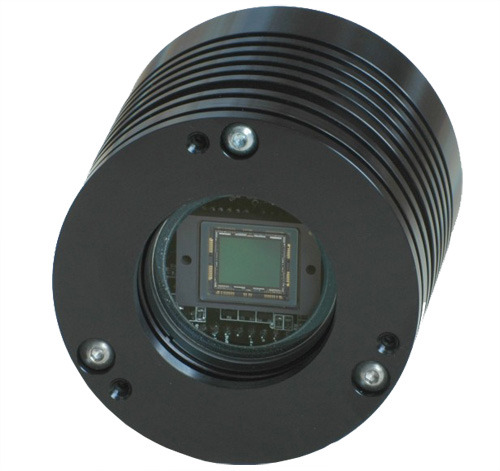
\includegraphics[width=0.6\textwidth]{../images/ccd.jpg}
		\caption[Cámara CCD]{Cámara CCD (\href{http://www.lunatico.es/}{http://www.lunatico.es/}).}
		\label{fig:ccd}
	\end{center}
\end{figure}

\bigskip
El \textbf{CCD} se inventó a finales delos 60 por investigadores de \textbf{Bell Laboratories}. Originalmente se concibió como un nuevo tipo de memoria de ordenador pero pronto se observó que tenía muchas más aplicaciones potenciales tales como el proceso de señales y sobretodo la captación de imagen, esto último debido a la sensibilidad a la luz que presenta el silicio.

\bigskip
El sensor \textbf{CCD} de una cámara digital es como el motor de un coche, es la pieza principal. En su forma más elemental, el \textbf{CCD} es como un ojo electrónico que recoge la luz y la convierte en una señal eléctrica. Tienen dos diferencias básicas con los foto-multiplicadores:

\bigskip
Los sensores \textbf{CCD} son de menor tamaño y están construidos de semiconductores lo que permite la integración de millones de dispositivos sensibles en un solo chip.
La eficiencia cuántica de los \textbf{CCD} (sensibilidad) es mayor para los rojos. Los foto-multiplicadores son más sensibles a los azules.

\bigskip
Físicamente, un \textbf{CCD} es una malla muy empaquetada de electrodos de polisilicio colocados sobre la superficie de un chip. Al impactar los fotones sobre el silicio se generan electrones generados que pueden guardarse temporalmente. Periódicamente se lee el contenido de cada píxel haciendo que los electrones se desplacen físicamente desde la posición donde se originaron (en la superficie del chip), hacia el amplificador de señal con lo que se genera una corriente eléctrica que será proporcional al número de fotones que llegaron al píxel. Para coordinar los periodos de almacenamiento (tiempo de exposición) y vaciado del píxel (lectura del píxel) debe existir una fuente eléctrica externa que marque el ritmo de almacenamiento-lectura: el reloj del sistema. La forma y amplitud de reloj son críticas en la operación de lectura del contenido de los píxeles.

\bigskip
Al tratarse el \textbf{CCD} de un dispositivo semiconductor, técnicamente es posible implementar en él todas las funciones electrónicas de un sistema de captación de imagen, pero esto no es rentable económicamente y por tanto se implementa en otros chips externos al \textbf{CCD}: la mayoría de \textbf{CCD} de cámaras tienen varios chips (de tres a ocho).

\bigskip
La necesidad de usar chips distintos implica dos desventajas importantes; la necesidad de voltajes múltiples de abastecimiento de los chips y un gran consumo de potencia de todo el sistema electrónico.


\subsection{Imágenes FITS}

En las imagenes astronómicas nos interesa almacenar la máxima cantidad de información sobre la imagen que tomamos, es por ello que siempre se usan formatos sin compresión, como puede ser RAW \cite{Raw} o FITS "Flexible Image Transport System"  \cite{FITS}.

\bigskip
\textbf{FITS} es un formato de imagenes especialmente concebido para el mundo de la astronomía, por permitir almacenar información más allá de la visible, así como espectros electromagnéticos.

\bigskip
Una característica muy interesante para los astrónomos es la incorporación de cabeceras en texto plano y legibles sin software adicional, en esta cabeceras se introducen \textbf{metadatos}, acerca del la observación,  posición geográfica, marcas de tiempo,  características de la cámara, filtros empleados entre otros.

\bigskip
FITS está soportado mediante bibliotecas disponibles en los lenguajes más utilizados en el ámbito científico, incluyendo C, FORTRAN, Java, Perl, PDL, Python, e IDL. 

\begin{figure}[h]
	\centering
	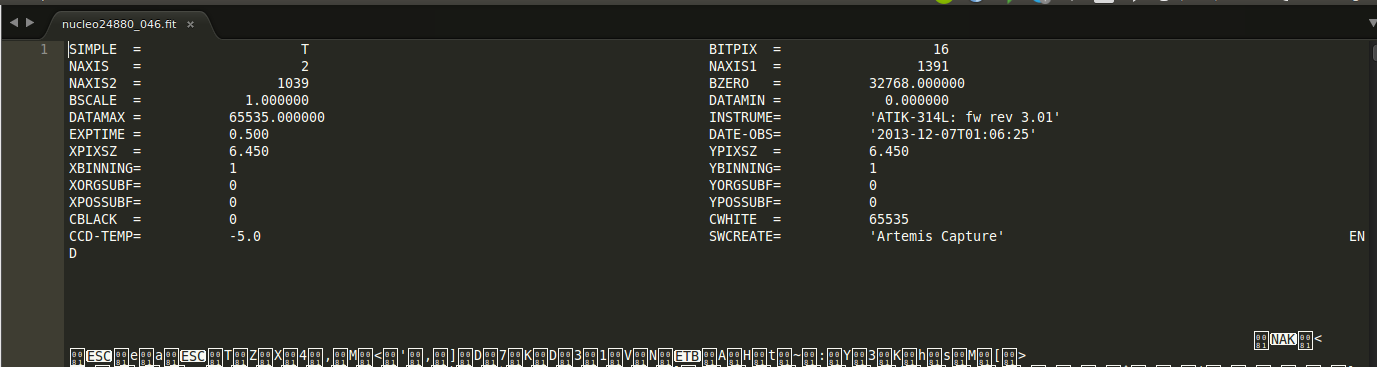
\includegraphics[width=1.0\linewidth]{../images/fit}
	\caption[Cabecera FITS]{Cabecera FITS}
	\label{fig:fit}
\end{figure}

\bigskip
Además existen numerosos entornos de procesamiento, que permiten manipular este tipo de imagenes, por nombrar uno de los más conocidos \textbf{ImageJ} \cite{Imagej}.


\subsection{Monturas}

La montura de un telescopio es la parte mecánica que une el trípode o base al instrumento óptico. Existen varios tipos de monturas, algunas muy simples, otras mas complejas, incluso con correctores electrónicos y dispositivos de localización y seguimiento muy sofisticados (sistemas \textbf{GOTO})

\bigskip
\begin{figure}[!ht]
	\begin{center}
		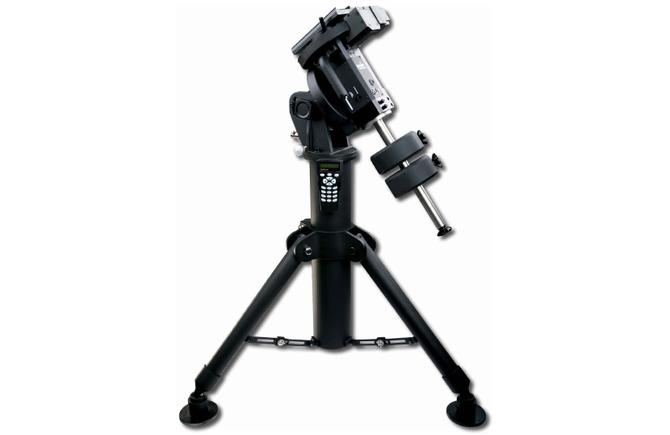
\includegraphics[width=0.6\textwidth]{../images/montura.jpg}
		\caption[Montura]{Montura (\href{http://tienda.lunatico.es/Montura-ecuatorial-SkyWatcher-EQ-8-con-tripod}{tienda.lunatico.es/Montura-ecuatorial}).}
		\label{fig:montura}
	\end{center}
\end{figure}

\bigskip
La montura tiene como objetivo proveer de movimiento controlado al telescopio.

\bigskip
Es muy importante la firmeza y suavidad de los movimientos, para que la observación sea confortable y las astro-fotografías perfectas. Las monturas se clasifican en dos grandes grupos, según los planos de referencia que utilicen (coordenadas).

\bigskip
La más simple es la montura \textbf{altacimutal}, que realiza movimientos horizontales y verticales (acimut y altura, respectivamente). Este tipo de diseño lo traen incorporados los telescopios pequeños, por lo general \textbf{telescopios refractores} de uso terrestre, dado que su uso es simple, y también varios modelos de equipos automatizados (sistemas \textbf{GOTO} )

\bigskip
Le sigue la \textbf{montura ecuatorial}, que utiliza como plano fundamental el ecuador celeste (proyección del ecuador terrestre). Este diseño usa las coordenadas ecuatoriales, ascensión recta (A.R. o R.A.) y declinación (Dec.), que son proyecciones de las coordenadas terrestres longitud y latitud, respectivamente, sobre la esfera celeste.


\subsection{Rueda portafiltros}

La rueda porta-filtros consiste en un cuerpo, generalmente de aluminio, que en su interior puede alojar varios \textbf{filtros}, normalmente de 1,25" de diámetro. Lo aconsejable es que tenga, al menos, 4 huecos para filtros para hacer astro-fotografía con cámaras CCD blanco y negro, puesto que se necesita  azul, rojo y verde (RGB) y, posiblemente, un filtro para infrarrojos.

\bigskip
Los mas comunes son los de colores, utilizados para resaltar las características de los objetos observados, sobre todo la atmosféricas y superficiales de los planetas.

\bigskip
Gracias a los filtros podemos fragmentar el espectro de luz, dejando pasar luz de una determinada longitud de onda, infiriendo características de los objetos.


\bigskip
\begin{figure}[!ht]
	\begin{center}
		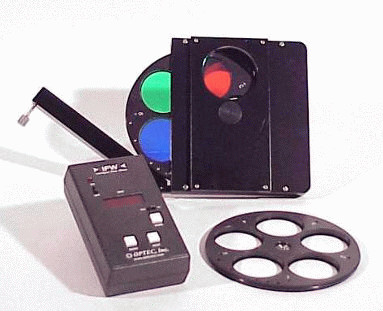
\includegraphics[width=0.3\textwidth]{../images/portafiltros.jpg}
		\caption[Rueda portafiltros]{Rueda portafiltros (\href{https://astroimagen.wordpress.com/productos/optec/ruedas-de-filtros-ifw/}{tienda.lunatico}).}
		\label{fig:portaf}
	\end{center}
\end{figure}



\subsection{Cúpulas}
Las \textbf{cúpulas} son recintos cerrados mas o menos grandes que nos permiten albergar y proteger el instrumental astronómico. De esta forma, las \textbf{cúpulas} pueden ser abiertas o cerradas para exponer los instrumentos en el momento de las observaciones.

\bigskip
\begin{figure}[!ht]
	\begin{center}
		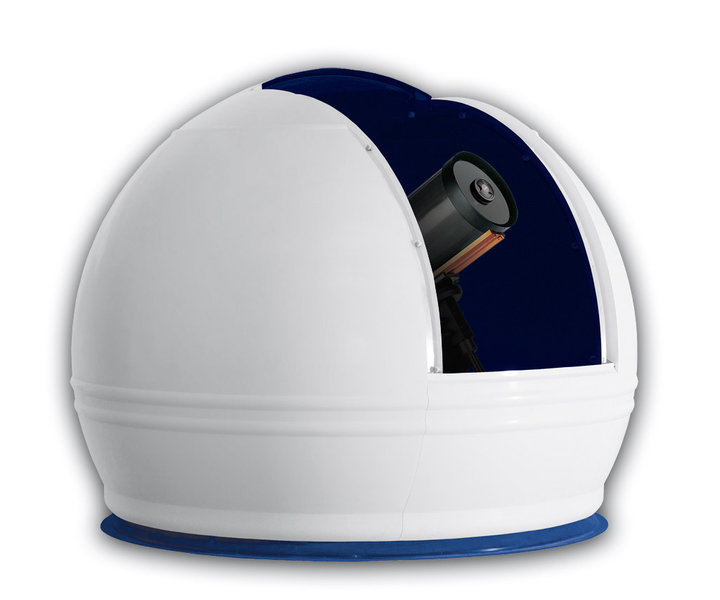
\includegraphics[width=0.3\textwidth]{../images/cupula.jpg}
		\caption[Cúpula]{Cúpula (\href{http://tienda.lunatico.es}{http://tienda.lunatico.es}).}
		\label{fig:diag_scrum}
	\end{center}
\end{figure}


\subsection{Estaciones meteorológicas}

Las \textbf{estaciones meteorológicas} son sistemas compuestos por un \textit{``data logger''} y un conjunto de sensores que nos proporcionan datos de las distintas magnitudes meteorológicas, tales como la temperatura, humedad, presión barométrica, etc... permitiéndonos generar modelos a partir de los cuales conocer la situación climática y su posible evolución. 

\bigskip
Gracias a los datos aportados por las \textbf{estaciones meteorológicas}, podemos conocer la climatología en el momento de realizar observaciones astronómicas. De esta forma podemos decidir si las condiciones son óptimas, o incluso decidir si debemos cerrar la cúpula para evitar daños en los instrumentos por lluvias o similar. 



\subsection{Enfocadores}

El \textbf{enfocador} es una pieza fundamental del telescopio que nos permitirá ver las imágenes formadas tras la reflexión de la luz en el espejo primario y su desviación por el espejo secundario.

En enfoque viene determinado por la convergencia de la mayor parte de los rayos justo en le plano focal, que es donde colocamos el ojo o una cámara. 

\begin{figure}[h]
\centering
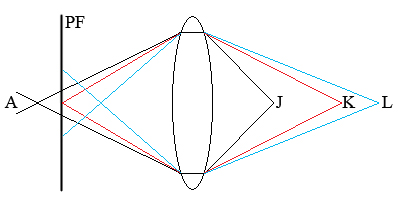
\includegraphics[width=0.7\linewidth]{../images/planofocal}
\caption{}
\label{fig:planofocal}
\end{figure}

\bigskip
El enfocador es una pieza adaptada al telescopio con una rueda dentada sobre una cremallera que podemos manipular para desplazar el portaocular unos centímetros y variar la distancia focal para encontrar el punto de foco óptimo.


\begin{figure}[h]
	\begin{center}
		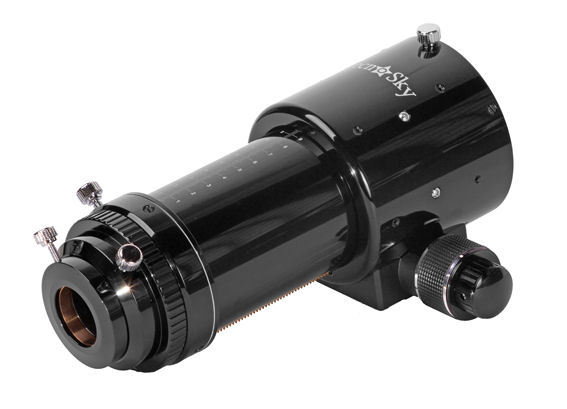
\includegraphics[width=0.4\textwidth]{../images/enfocador.jpg}
		\caption[Enfocador]{Enfocador (\href{http://tienda.lunatico.es}{http://tienda.lunatico.es}).}
		\label{fig:diag_scrum}
	\end{center}
\end{figure}


\bigskip
Como en observación astronómica se suele trabajar a muchos aumentos un pequeño error de enfoque se magnifica traduciéndose enseguida en una imagen poco nítida o desenfocada.


\bigskip
Para ayudar en esta operación los astrónomos han perfeccionado algunas técnicas, una de las más extendidas es hacer uso de una máscara de enfoque. \cite{FocusMascara}

\bigskip
Que no es más que unas rendijas por las que hacemos pasar la luz de un objeto luminoso, difractando los rayos y observando la dirección que toman.


\bigskip
Otra característica que incorporan muchos enfocadores comerciales es la \textbf{comprensión por temperatura}, para ello incorpora un sensor en la óptica, que informa de grandes oscilaciones en la temperatura, (que puedan producir dilatación en la lente), 
cuando se detecta una oscilación considerable en la temperatura, se ejecuta un ciclo de autoenfoque, (o se compensa según alguna regla establecida).


\subsection{Enfoque asistido por ordenador}

Una técnica muy extendida entre los astrónomos es el uso de \textbf{software} especializado, que mediante un procesamiento de imagenes es capaz de obtener una medida de la nitidez del objeto y compararlo con el valor óptimo.

\bigskip
Dado que es una de los puntos clave del \textbf{scope} del proyecto, no paro a profundizar dado que más adelante enterremos en detalle en la explicación de las medidas, algoritmos, así como las implementaciones.  


\newpage
\section{Control remoto de dispositivos astronómicos}

En la actualidad se están implantando cantidad de protocolos y estándares de manejo remoto, al campo de la astronomía, por varios  motivos como agilizar y facilitar la observación, librar al astrónomo de tareas tediosas, soportar condiciones climatológicas adversas y permitirle centrarse en la propia observación así como multiplicar el numero de puestos dado que un equipo de astrónomos puede controlar varios observatorios desde remoto, mientras que de forma física se ven limitados a uno solo. 

\begin{figure}[h]
\centering
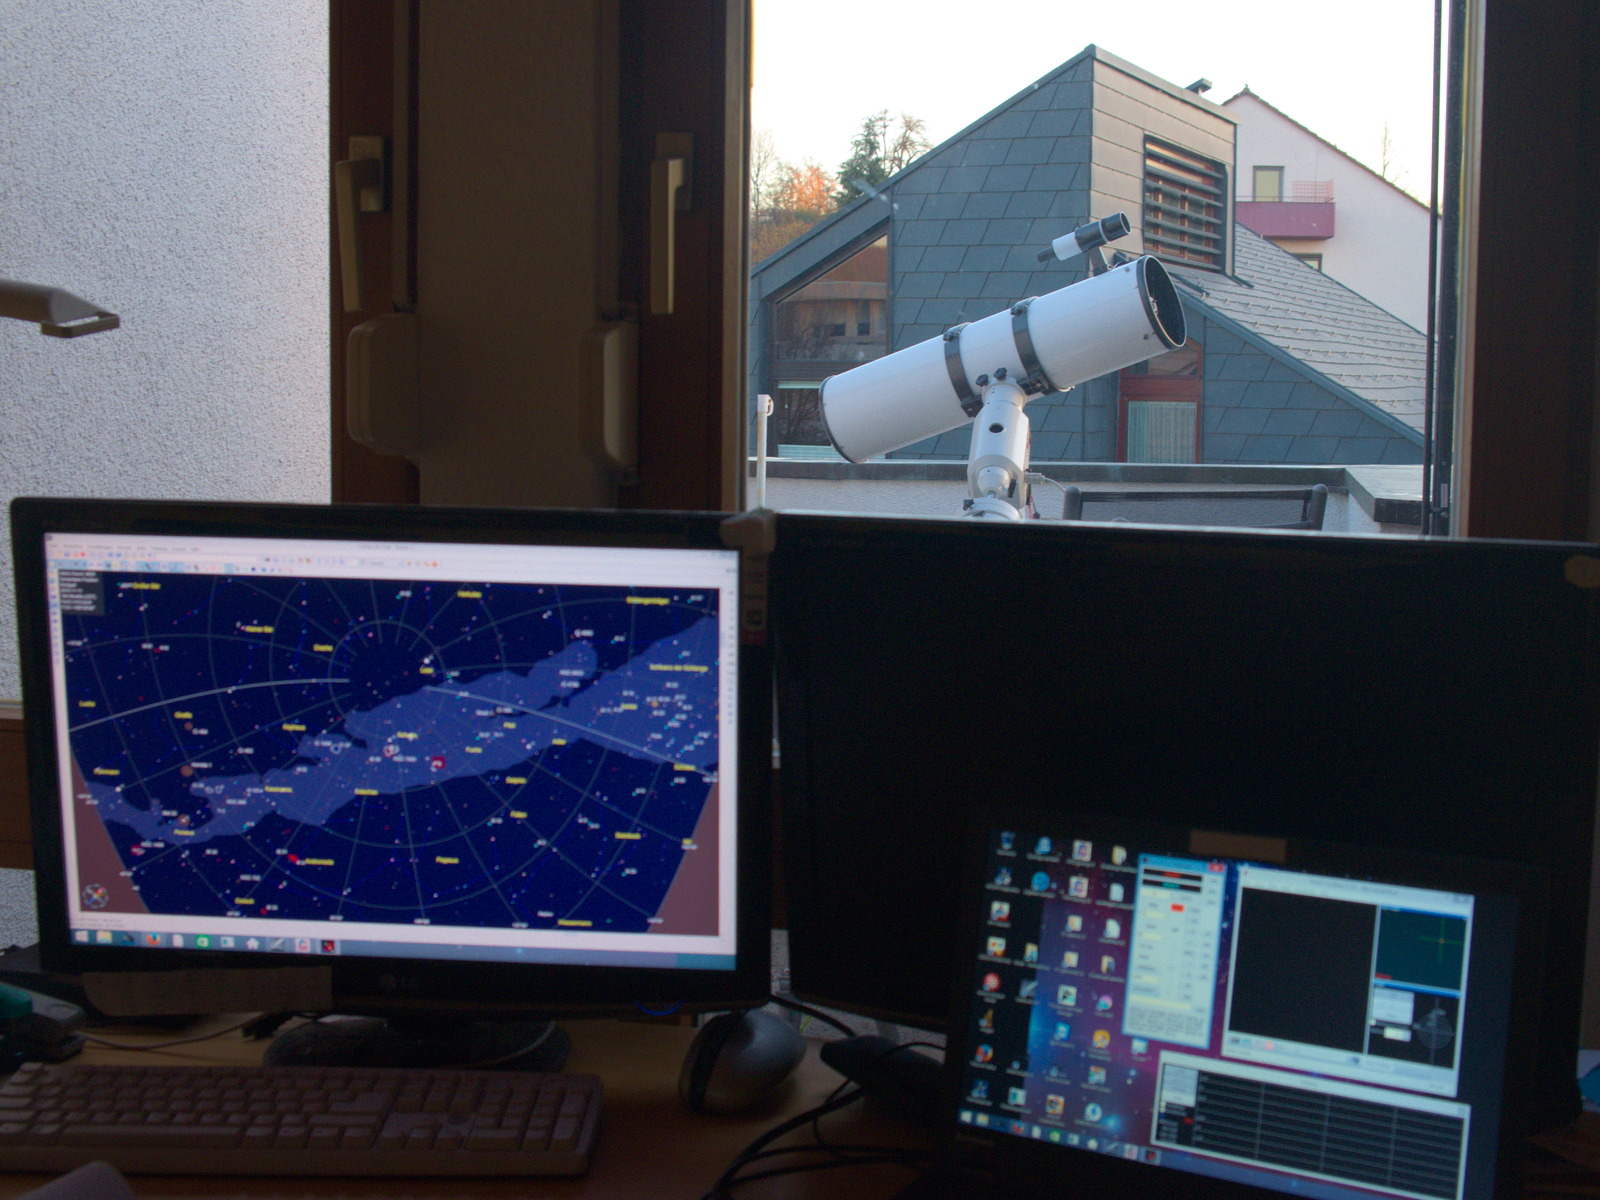
\includegraphics[width=0.7\linewidth]{../images/robotizacion}
\caption{}
\label{fig:robotizacion}
\end{figure}

Actualmente existen diversas formas de controlar los dispositivos astronómicos pero la mayoría presenta los mismos inconvenientes:

\begin{itemize}
	\item Normalmente se controlan los dispositivos directamente.
	\item Se conecta el dispositivo a un PC y se trabaja desde él.
	\item Se utilizan herramientas para el control remoto como el escritorio remoto.
\end{itemize}

\newpage

La evolución de las plataformas se puede resumir:

\begin{enumerate}
\item Esquema monolítico:  Cada dispositivo, funciona con us propio cliente y usa su protocolo particular.

\item Esquema extensible: Donde algunos vendedores comparten el código de control, pero es un circulo cerrado y nadie de forma independiente puede implementar nuevos plugins.

\item ASCOM, intenta crear una capa entre los programas para controlar dispositivos astronómicos y los propios dispositivos, dado que es un estándar abierto, cualquiera puede implementar nuevos driver para sus dispositivos, por contrapunto solo puede utilizarse en sistemas \textit{Microsoft Windows}. Su diseño tiene una relación bastante profunda con el sistema operativo lo cual dificulta el desarrollo basado en red.

\item INDI, es más abierto que el anterior y dispone de múltiples implementaciones en C y  Java \cite{indiforjava}, se puede desplegar en en cualquier sistema operativo, ya sea Windows, Linux o Mac.

\end{enumerate}

\section{INDI}

\begin{quote}``\textit{The Instrument Neutral Distributed Interface (INDI) Library is a cross-platform software designed for automation  control of astronomical instruments. It supports a wide variety of telescopes, CCDs, focusers , filter wheels..etc, and it has the capability to support virtually any device. INDI is small, flexible, easy to parse, and scalable. It supports common DCS functions such as remote control, data acquisition, monitoring, and a lot more. With INDI, you have a total transparent control over your instruments so you can get more science with less time.}''
	\newline(\href{http://indilib.org/about.html}{http://indilib.org/about.html})
\end{quote}

\bigskip
El protocolo \textbf{INDI} es una plataforma software diseñada para el control de instrumental astronómico, aunque podría usarse con cualquier dispositivo, incluidos ``virtuales''. La biblioteca \textbf{INDI} permite controlar cualquier dispositivo con un driver \textbf{INDI} mediante el paso de archivos XML. Sus principales ventajas frente a otras soluciones para el control de dispositivos son:


\begin{itemize}
	\item Es una biblioteca ligera, flexible y escalable.
	\item Es de código abierto por lo que cualquiera puede ver su código y mejorarlo o crear drivers para cualquier dispositivo.
	\item El intercambio de información entre clientes, servidores y drivers es mínimo.
	\item Es multiplataforma.
	\item Separa clara y totalmente el cliente del servidor.
	\item Los fabricantes comienzan a desarrollar drivers para sus dispositivos o liberan las especificaciones para que la comunidad pueda desarrollarlos.
	\item Existen numerosos clientes INDI como \href{https://edu.kde.org/kstars/}{kstars}, Cartes Du Ciel, Xephem y Stellarium (en fase de desarrollo).
	
\end{itemize}


\bigskip

\subsection{Breve introducción a INDI}

INDI consiste a su nivel más básico en un protocolo que permite el control, automatización, obtención de datos e intercambio de los mismos entre distintos dispositivos hardware y programas cliente. La idea subyacente en el protocolo INDI es desacoplar aspectos específicos del hardware que se controla de tal manera que cambios en el hardware no impliquen necesariamente cambios en el software (cosa que ocurre en sistemas más habituales donde el el frontend software está fuertemente acoplado con el backend hardware.

\bigskip
\begin{figure}[!ht]
	\begin{center}
		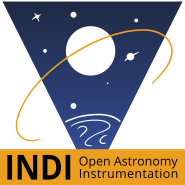
\includegraphics[width=0.21\textwidth]{../images/indi.png}
		\caption[INDI Lib]{INDI Lib (\href{http://indilib.org/}{http://indilib.org/})}
		\label{fig:ascom}
	\end{center}
\end{figure}


\bigskip
Para conseguir un desacople efectivo entre los clientes y el hardware se define un protocolo basado en XML que permite abstraer los dispositivos hardware como conjuntos de propiedades que pueden ser leídas, y modificadas por los clientes (siempre estableciendo las restricciones oportunas).


\subsection{Drivers, Servidores y Clientes INDI}

Pese a que nivel más básico INDI es ``simplemente'' una especificación de un protocolo basado en XML, a un nivel superior se distinguen tres entidades diferentes que interaccionan entre sí para tener un sistema de control plenamente funcional:

\begin{itemize}
	\item \textbf{Drivers:} Son programas que se ejecutarán en la máquina en la que están conectados los dispositivos hardware. Son los encargados de la comunicación directa con los dispositivos y su abstracción a propiedades INDI.
	
	\item \textbf{Servidor:} Es un programa cuya función principal es ejecutar los drivers y permitir la conexión a los mismos por parte de los clientes (funciona de un modo similar a un proxy). Normalmente reside en la máquina donde están conectados los dispositivos, aunque en principio se pueden crear estructuras de red tipo árbol de servidores. El intercambio de información entre el servidor y los drivers se realiza utilizando el protocolo INDI.
	
	\item \textbf{Cliente:} Es un programa que permite conectar con uno o más servidores y su función principal e hacer de interfaz con el usuario. Para ello conecta (usualmente a través de la red) con el servidor e intercambia información sobre los dispositivos utilizando el protocolo INDI. Es interesante recalcar que los clientes pueden ser de cualquier estilo: desde programas con interfaz de usuario avanzadas, hasta programas simples en línea de comandos scripts completamente automáticos que controlen o monitoricen los dispositivos.
\end{itemize}



La biblioteca \textbf{INDI} está escrita en lenguaje \textbf{C}, pero existe una implementación completa realizada en \textbf{Java} y que se encuentra en constante mejora. En la página oficial de \href{http://indilib.org/develop/indiforjava.html}{INDI}} podemos encontrar toda la información sobre nuevas versiones y la documentación para poder utilizarla. La principal ventaja de poder usar \textbf{Java} es que podemos implementar drivers y clientes con la potencia de un lenguaje Orientado a Objetos y combinarlo con otras tecnologías como los dispositivos móviles basados en la plataforma \textbf{Android}


\bigskip

\newpage

\section{Hardware Libre}


Se llama hardware libre, hardware de código abierto, electrónica libre o máquinas libres a aquellos dispositivos de hardware cuyas especificaciones y diagramas esquemáticos son de acceso público, ya sea bajo algún tipo de pago, o de forma gratuita. La filosofía del software libre es aplicable a la del hardware libre, y por eso forma parte de la cultura libre. \cite{HWLIBRE}

Problemas que trata de solventar el hardware libre:

\bigskip
1.) Conocimiento lo poseen las empresas.
	Haciendo público todos la documentación, diagramas, data shield, fichas etc.

\bigskip
2.) Falta de materiales o herramientas para la fabricación.
	Tratan de utilizar componentes estándar, que se puedan encontrar fácilmente. 
	Así como hacer recomendaciones de algunas tiendas online donde puedes comprar tales componetes.  

\bigskip
3.) Altos costes de producción.
	Al ser de diseño libre, diferentes factorías pueden ocuparse de fabricar los componentes, preocupandondose por optimizar y agilizar el proceso, llegando a bajar los costes de producción.

 \bigskip
4.) Gran inversión en realizar trabajos redundantes. 
	No hay que preocuparse por solucionar una y otra vez los mismo problemas, para nuestros diseños podemos partir de una buena base.


Dado este movimiento han surgido muchísimas plataformas, pero en especial cabe remarcar dos de las más importantes. 

\newpage
\subsection{Arduino}


\begin{figure}
\centering

\includegraphics[width=0.5\linewidth]{../images/arduino}
\caption[Arduino]{Arduino (\href{https://www.arduino.cc/})}
\label{fig:arduino}
\end{figure}


\bigskip
\paragraph{Arduino} es una compañía de hardware libre, la cual desarrolla placas de desarrollo que integran un \textbf{microcontrolador} y un entorno de desarrollo  \cite{IDE}.

\bigskip
Diseñado para facilitar el uso de la electrónica en proyectos multidisciplinarios. \cite{ARDUINO}

\bigskip
La primer placa Arduino fue introducida en el 2005, ofreciendo un bajo costo y facilidad de uso para novatos y profesionales buscando desarrollar proyectos interactivos con su entorno mediante actuadores y sensores.

\bigskip
A partir de Octubre del año 2012, se incorporaron nuevos modelos de placas de desarrollo que hacen uso de microcontroladores \textbf{CortexM3}, \textbf{ARM}.

\bigskip
Tal como marcan los principios del hardware libre, los esquemáticos de diseño del Hardware están disponibles bajo licencia Libre, permitiendo a cualquier persona crear su propia placa Arduino sin necesidad de comprar una prefabricada. 


\begin{figure}[h]
	\centering
	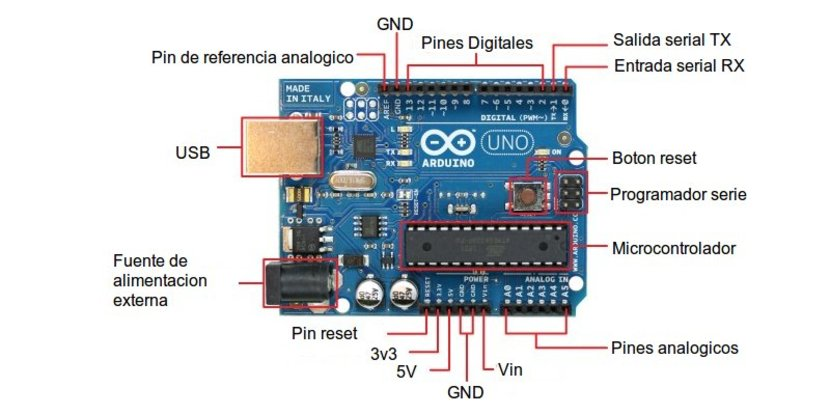
\includegraphics[width=0.7\linewidth]{../images/caracteristicas_arduino}
	\caption[Arduino Casero]{Arduino Casero (\href{http://www.cerosecurity.com/como-construir-un-arduino-casero/})}
	\label{fig:arduinocasero}
\end{figure}


\textbf{Modelos de Arduino}  \\

Existen multitud de ediciones o modelos de placa, cada una pensada para un público concreto o para una serie de tareas o proyectos específicos. También han surgido muchos modelos nó oficiales. 

\bigskip
Muchas veces las diferencias son sutiles, pero en otras ocasiones las diferencias entre placas son mucho más considerables y una buena elección puede condicionarnos completamente en desarrollo, así como una mala elección nos puede limitar completamente. 

Por nombrar algunas placas de las más famosas:
\begin{itemize}
	
\item \textbf{Arduino UNO}: es la plataforma más extendida y la primera que salió al mercado.

\item \textbf{Arduino TRE}: Procesador de alta potencia, AM335x de 1Ghz.

\item \textbf{Arduino/Genuino 101}: Módulo Intel Curie, de dimensiones reducidas y bajo consumo potenciados por el SoC Intel Quark de 32 bits.

\item \textbf{Arduino Yun}: Combina un chip ATmega32u4 y en un chip Atheros AR9331, que se comunican mediante un puente. El chip Atheros soporta distribuciones ligeras de Linux. 

\item \textbf{Arduino Mega}: Incorpora un chip ATmega2560, dando más rendimiento que el ATmega320 del Arduino UNO

\item \textbf{Arduino Ethernet}: Identico al Arduino UNO, pero con conexión a red.

\item \textbf{Arduino Nano y Micro y TinyDuino}: De muy pequeño tamaño y optimizadas para mejorar el consumo. 

\item \textbf{Arduino LilyPad}: está pensado para insertarse en prendas y textiles, es lavable. 

\end{itemize}


\textbf{Shields para Arduino} \\ 

Son placas de circuitos modulares que se montan unas encima de otras para dar funcionalidad extra a un Arduino.

\bigskip
Las shields se pueden comunicar con el arduino bien por algunos de los pines digitales o analógicos o bien por algún bus como el SPI, I2C o puerto serie, así como usar algunos pines como interrupción. Además estas shields se alimenta generalmente a través del Arduino mediante los pines de 5V y GND. \cite{shield}

\bigskip
Podemos destacar algunos de los shield más comunes y recomendables para multitud de proyectos, \textbf{Arduino Wifi Shield}, que añade comunicación wireless WIFI, \textbf{Arduino GSM Shield}, añade comunicación GPRS, usando una tarjeta SIM,
\textbf{Arduino Motor Shield}, permite manejar motores DC, \textbf{GPS Shield}, añade localización GPS, \textbf{Xbee Shield}, comunicación inalámbrica XBee \cite{XBee}, entre muchos otros. 


\begin{figure}[h]
\centering
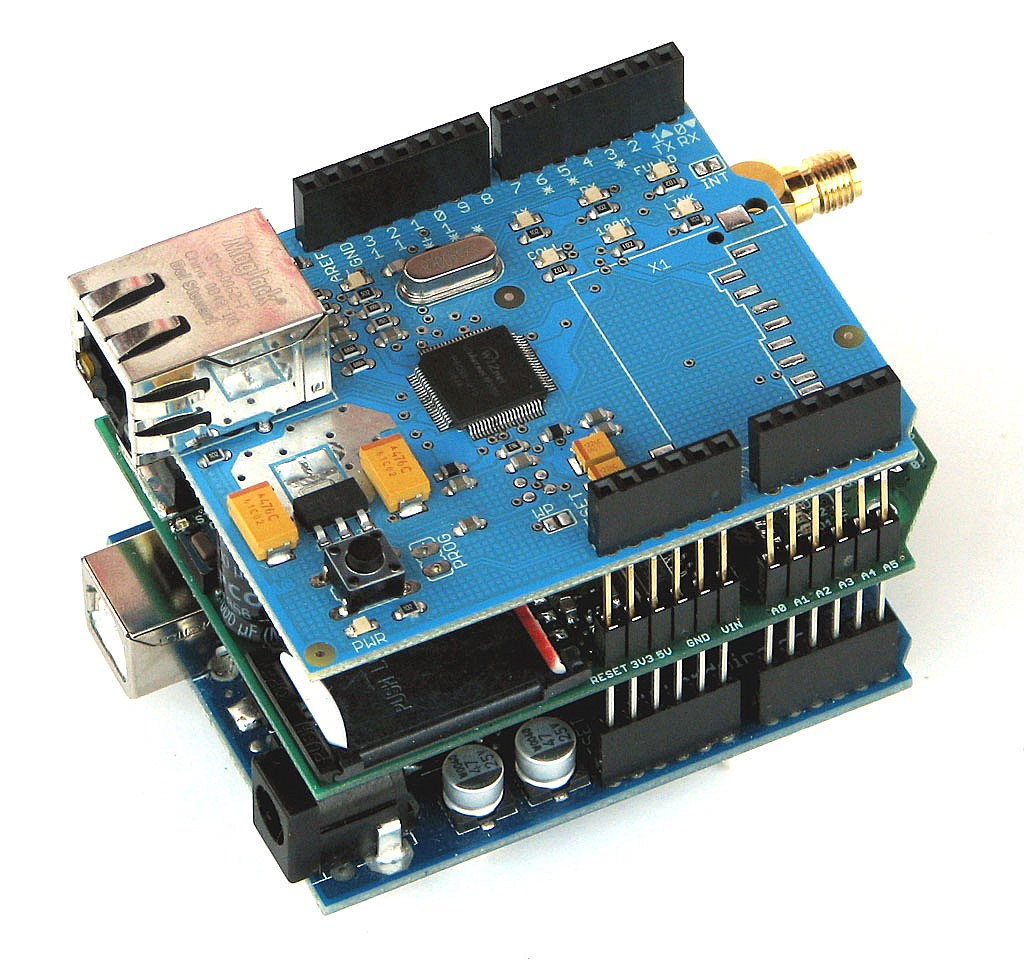
\includegraphics[width=0.4\linewidth]{../images/arduinoshield}
\caption{}
\label{fig:arduinoshield}
\end{figure}

\newpage


\paragraph{Framework desarrollo Arduino:}

El lenguaje de programación de Arduino (basado en Wiring) e implementado en C++.

\bigskip
Posee su propio entorno de programación, con opciones para compilar y cargar el código fuente en la placa que tenemos conectada.

\begin{figure}[h]
\centering
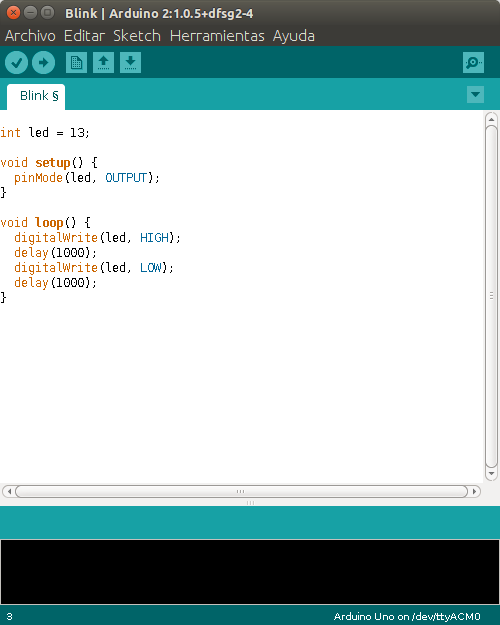
\includegraphics[width=0.4\linewidth]{../images/arduinoide}
\caption{}
\label{fig:arduinoide}
\end{figure}

Por otro lado también podemos encontrar multitud de librerías y módulos ya implementados, que se pueden incorporar directamente a nuestros proyectos, realizando algunas abstracciones sobre el hardware, comunicación o algún aspecto de más bajo nivel.

\bigskip
\url{http://www.arduino.cc/en/Reference/Libraries}
\href{http://www.arduino.cc/en/Reference/Libraries}{ }

\newpage

\subsection{Raspberry Pi}

En el mundo del hardware libre encontramos otro protagonista,
\textbf{Raspberry Pi}, aunque su libertad es algo más limitada que la anterior, al ser propiedad registrada, pero de uso libre.

\bigskip
Cuenta con procesadores ARM y una GPU, así como una limitada meroría RAM, permitiendo instalar un sistema operativo completo y correr algunos script. 

\bigskip
Existiendo distribuciones especialmente compiladas, Raspbian (derivada de Debian), RISC OS 5, Arch Linux ARM (derivado de Arch Linux) y Pidora (derivado de Fedora).

\bigskip
Dispone de una serie de pines para propósito general, con los cuales podemos activar señales para controlar algunos dispositivos, por lo cual es una placa también usada en domotica.

\bigskip
Han salido varias evoluciones de la placa, pasando por las Pi 1 A, Pi 1 B y B+, Pi 2 B, Pi 3 esta última incorporando un procesador ARMv8 de 64 bits, a 1.2GHz que proporciona unas prestaciones más que razonables para montar un pequeño servidor de aplicaciones. 

El proyecto que presento es un claro ejemplo pues instalo el servidor de control remoto del observatorio una maquina de este tipo.


\begin{figure}[h]
\centering

\includegraphics[width=0.2\linewidth]{../images/raspberry}
\caption[Raspberry Pi]{Raspberry Pi}
\label{fig:raspberry}
\end{figure}




  